%----------------------------------------------------------------------------------------
%	PACKAGES AND DOCUMENT CONFIGURATIONS
%----------------------------------------------------------------------------------------

\documentclass{article}

\usepackage{graphicx} % Required for the inclusion of images
\usepackage{subfigure} % Required for the inclusion of images
\usepackage{natbib} % Required to change bibliography style to APA
\usepackage{amsmath} % Required for some math elements
\usepackage{titlesec}
\usepackage[usenames]{xcolor}
\usepackage{subfig}
\usepackage{float}
\usepackage{listings}
\definecolor{mygreen}{rgb}{0,0.6,0}
\definecolor{mygray}{rgb}{0.5,0.5,0.5}
\definecolor{mymauve}{rgb}{0.58,0,0.82}
\lstset{
 backgroundcolor=\color{lightgray},
 basicstyle = \footnotesize,
 breakatwhitespace = false,
 breaklines = true,
 captionpos = b,                    
 %commentstyle = \color{mygreen}\bfseries,
 extendedchars = false,
 frame =shadowbox,
 framerule=0.5pt,
 keepspaces=true,
 %keywordstyle=\color{blue}\bfseries, % keyword style
 language = Verilog,      % the language of code
 otherkeywords={string},
 numbers=left,
 numbersep=5pt,
 numberstyle=\tiny\color{mygray},
 rulecolor=\color{black},
 showspaces=false,
 showstringspaces=false,
 showtabs=false,
 stepnumber=1,
 stringstyle=\color{mymauve},        % string literal style
 tabsize=4,
 title=\lstname
}


\setcounter{secnumdepth}{4}

\titleformat{\paragraph}
{\normalfont\normalsize\bfseries}{\theparagraph}{1em}{}
\titlespacing*{\paragraph}
{0pt}{3.25ex plus 1ex minus .2ex}{1.5ex plus .2ex}



%\usepackage{times} % Uncomment to use the Times New Roman font

%----------------------------------------------------------------------------------------
%	DOCUMENT INFORMATION
%----------------------------------------------------------------------------------------

\title{\textbf{Project 1: Optimizing the Performance of a Pipelined Processor}} % Title

\author{
        516021910127, Yifeng Gao, xdek@msn.com \\
        515021910302, Chacha Chen, chachachen1997@gmail.com \\
        516021910495, Zhixin Ling, 1069066484@qq.com, group leader } % Author name and email

\date{\today} % Date for the report

\begin{document}


\maketitle % Insert the title, author and date

\section{Introduction}

Throughout this lab, we learned about the design and implementation of a pipelined Y86 processor, optimizing both it and a benchmark program to maximize performance. After this lab, not only did we all have a keen appreciation for the interactions between code and hardware that affect the performance of your programs, but also became more familier with linux operations and computer architecture etc.

In part A, we implemented 3 basic functions using assembly language and in part B, we implemented new instructions iaddl and leave in the sequence processor and apply iaddl to our Y86 assembly programs. In part C, we implemented new instructions iaddl and leave in the pipeline processor and optimized a program with some optimization techniques and iaddl instruction.

\noindent\textbf{Arrangement:}
Zhixin Ling, as the group leader, finished Part C and the corresponding report section. Chacha Chen and Yifeng Gao work cooperatively on Part A and Part B as well as the corresponding report section and the integration of the report and final hand-in directories.


\section{Experiments}
The experiment includes 3 parts.

\subsection{Part A}

\subsubsection{Analysis}
\begin{itemize}
\item \textbf{sum.ys}
 is a program that iteratively sums the elements of a linked list. 

The basic idea is that we use a conditional jump in a loop which iteratively check whether the next element is equal to zero and if not add up the value to the sum.

\begin{itemize}
\item In init part, the stack structure is set up, then the program jumps to Main function, and finally halts.
\item In Main, we first store the first element to the stack before a call to function sum\_list. 
\item In sum\_list function, we first do the conventions which saves a copy of initial \%ebp and set \%ebp to the beginning of the stack frame. Then we initialize the sum=0, and the go to a loop which iteratively add up elements' value into our sum. 
\item In loop: firstly, the element pointed to is added and then, we increment the pointer address which make it points to the next element. If the next element is equal to zero, jump to done, otherwise loop agian. 
\item In done: we resume the \%esp and \%ebp to the initial value set in init part. Then we can safely let Main function return.
\end{itemize}

\item \textbf{rsum.ys}
is a program that recursively sums the elements of a linked list. 

This most of the code is similar to the code in sum.ys, except that it should use a function rsum list that recursively sums a list of numbers. 

\begin{itemize}
\item In rsum\_list, the key idea is that we use \%eax to store the iterative temporary sum meanwhile store the value of the current element in \%edx. Also, a very important point is that we should store the address of the next element(if it is not zero) always in 8(\%ebp), such that in every recursive step, we always update the desired element, which in this case we update $element[i+1]$ with the sum of all elements from $i+1$ to the end.
\end{itemize}
\item \textbf{copy.ys} copies a block of words from one part of memory to another (non-overlapping area) area of memory, computing the checksum (Xor) of all the words copied.

\begin{itemize}
\item The initialization step is similar to the above implementations.
\item In Main: firstly, the store the src, dest and len into main function stack frame for future use. After these preliminaries, copy block function is called. After returning from copy block, we need to resume the esp and ebp to the initial value set in init part and this is done by "done" function part as similar to above implementations. Finally Main function is returned.
\item copy\_block: In copy block, firstly we do the conventions like saving a copy of caller’s ebp and set ebp to the beginning of copy block ’s stack frame. Then we use 3 registers \%ebx \%ecx, \%esi to store temporary needed values for iteration. Also, \%eax, the stored length, is subtracted by 1 and a conditional jump instruction was added to terminated the loop when the length is equal to zero. In each iteration, we copy the value stored in the current source block to the current destination block. The addresses of both is calculated by a increment factor \%esi added to the current address(\%edx for src and \%ebc for dest).

Finally, we resume the esp and ebp and return.
\end{itemize}

\end{itemize}
\subsubsection{Code}
\begin{itemize}
\item \textbf{sum.ys}
  \begin{lstlisting}[caption={}]
#Execution begins at address 0
	.pos	0			#start address for all Y86 programs
Init:
	irmovl	Stack, %esp		#Initialize stack pointer
	irmovl	Stack, %ebp		#Initialize base pointer
	jmp	Main
	halt

.align	4
ele1:					#Elements initialization
		.long 0x00a
		.long ele2
ele2:
		.long 0x0b0
		.long ele3
ele3:	
		.long 0xc00
		.long 0

Main:
		irmovl	ele1,%esi	#starting pointer
		pushl	%esi
		call sum_list	
		halt

sum_list:
		pushl	%ebp
		rrmovl	%esp, %ebp	#read the stack pointer
		mrmovl	8(%ebp),%ebx	#ebx = start pointer ele1
		irmovl	$0,%eax		#sum=0
loop:		mrmovl	(%ebx),%edx	#The element
		addl	%edx,%eax
		mrmovl	4(%ebx), %esi	#4(%ebx) is address of next node
		andl 	%esi, %esi 	#if %esi=zero,jump to done
		je		done	#If the pointer points to zero, return
		rrmovl	%esi,%ebx
		jmp		loop
done:		popl	%esi		#restore the registers
		popl	%edx
		popl	%ebx
		rrmovl	%ebp, %esp
		popl	%ebp
		ret  
#stack starts here and grows to lower addresses
		.pos	0x400
Stack:

 \end{lstlisting}


\item \textbf{rsum.ys}
  \begin{lstlisting}[caption={}]
 #Execution begins at address 0
	.pos	0
Init:
	irmovl	Stack, %esp		#Initialize stack pointer
	irmovl	Stack, %ebp
	jmp		Main
	halt

.align	4
ele1:
		.long 0x00a
		.long ele2
ele2:
		.long 0x0b0
		.long ele3
ele3:	
		.long 0xc00
		.long 0


Main:
		irmovl	ele1,%esi	#p_ele1
		pushl	%esi
		xorl    %eax, %eax	#set eax=0
		call rsum_list	
		halt

rsum_list:
		pushl	%ebp
		rrmovl	%esp, %ebp	#read the stack pointer
		pushl	%ebx		#save ebx
		pushl	%ecx		#save ecx
		pushl	%edx		#save edx
		pushl	%esi		#save esi
		mrmovl	8(%ebp),%edx	#edx=p_ele[i]
		mrmovl	0(%edx),%eax	#eax=ele[i]
		mrmovl	4(%edx),%ebx	#ebx=p_ele[i+1]
		andl	%ebx, %ebx	#if p_ele[i+1] == 0
		je  	done		#return ele[i]
		pushl	%ebx		#else: 8(%ebp)=p_ele[i+1]
		rrmovl  %eax, %ecx	#ecx = ele[i]
		call 	rsum_list
		popl	%edx		#restore the stack pointer
		addl	%ecx,%eax	#eax += rsum(p_ele[i+1])
done:					#return
		popl	%esi			#restore the registers
		popl	%edx
		popl 	%ecx
		popl	%ebx
		rrmovl	%ebp, %esp
		popl	%ebp
		ret

		.pos	0x120
Stack:
 


\end{lstlisting}

\item \textbf{copy.ys}
  \begin{lstlisting}[caption={}]
#Execution begins at address 0
	.pos	0
Init:
	irmovl	Stack, %esp			#Initialize stack pointer
	irmovl	Stack, %ebp
	jmp	Main
	halt

.align	4
src:
	.long	0x00a
	.long	0x0b0
	.long	0xc00
dest:
	.long	0x111
	.long	0x222
	.long	0x333


Main:
		irmovl	src,%esi		#src
		pushl	%esi
		irmovl	dest,%esi		#dest
		pushl	%esi
		irmovl	$3,%esi			#len
		pushl	%esi
		call copy_block	
		halt

copy_block:
		pushl	%ebp
		rrmovl	%esp, %ebp		#read the stack pointer
		pushl	%ebx			#save ebx
		pushl	%ecx			#save ecx
		pushl	%edx			#save edx
		pushl	%esi			#save esi
		mrmovl	8(%ebp),%eax		#eax=len,len-1,...,0
		irmovl	$0,%ebx			#tmp=0
		irmovl	$0,%ecx			#ecx=0
		irmovl	$0,%esi			#esi=0,4,8...
loop:	
		mrmovl	16(%ebp),%edx		#edx = p_src
		addl	%esi,%edx		#edx = p_src_cur
		mrmovl	0(%edx),%edx		#edx = src_cur
		xorl	%edx,%ecx		#result ^= src_cur

		mrmovl	12(%ebp),%ebx		#ebx = p_dest
		addl	%esi,%ebx		#ebx = p_dest_cur
		rmmovl	%edx,0(%ebx)		#*p_dest_cur = src_cur

		irmovl  $1,%ebx			#eax-=1
		subl	%ebx,%eax		#subl	%ebx,%eax -> eax = eax - ebx
		je		done
		irmovl	$4,%ebx			#tmp = 4
		addl	%ebx,%esi		#esi+=tmp
		jmp		loop
done:		rrmovl	%ecx,%eax
		popl	%esi			#restore the registers
		popl	%edx
		popl 	%ecx
		popl	%ebx
		rrmovl	%ebp, %esp
		popl	%ebp
		ret

		.pos	0x120
Stack:

\end{lstlisting}
\end{itemize}


\subsubsection{Evaluation}


\begin{itemize}
\item \textbf{sum.ys}

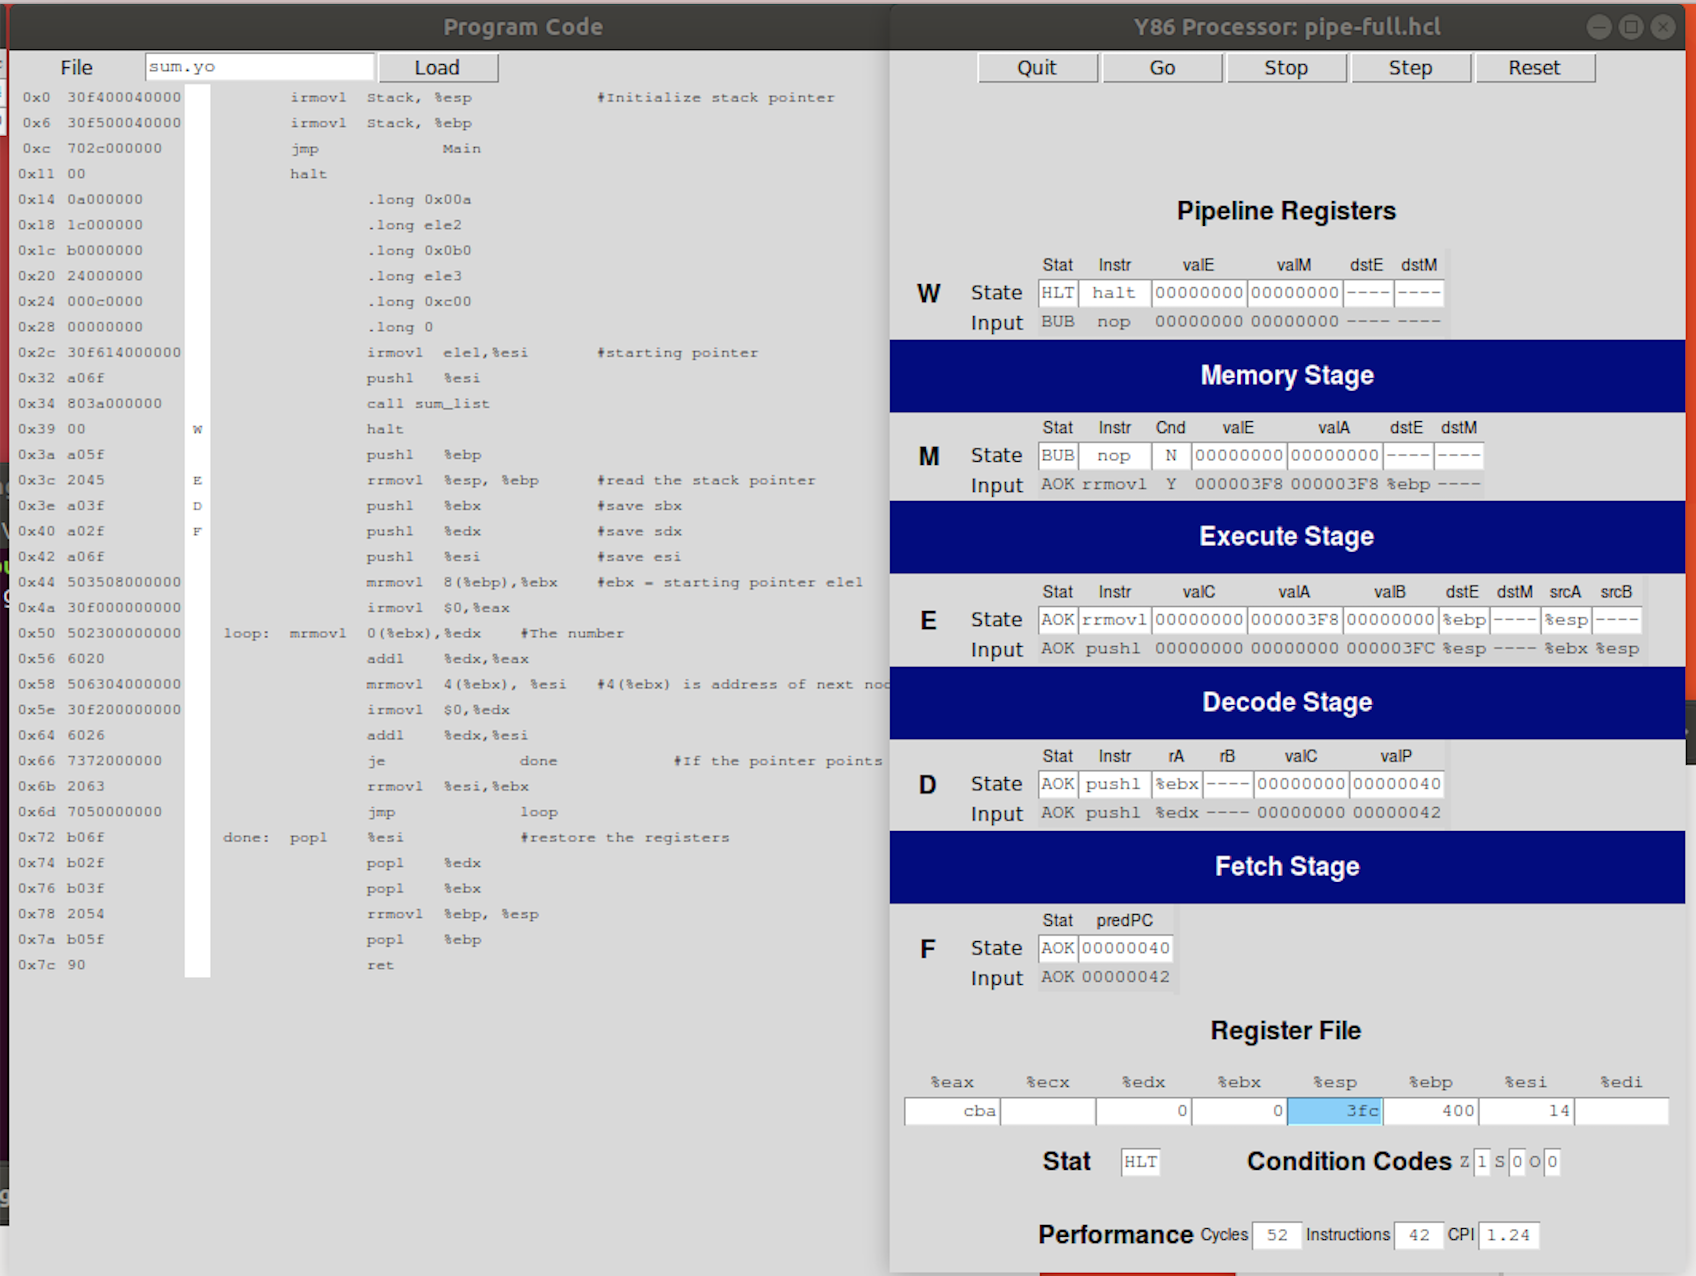
\includegraphics[width=0.95\textwidth]{A-sum.png}
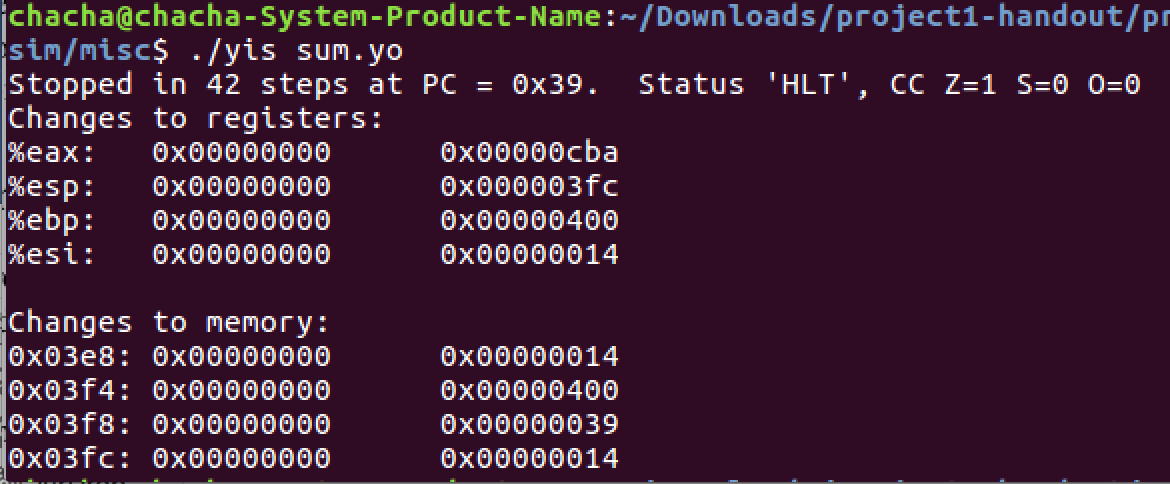
\includegraphics[width=0.95\textwidth]{sum.png}
As is shown above, our implementation can be seen as successful.

\item \textbf{rsum.ys}

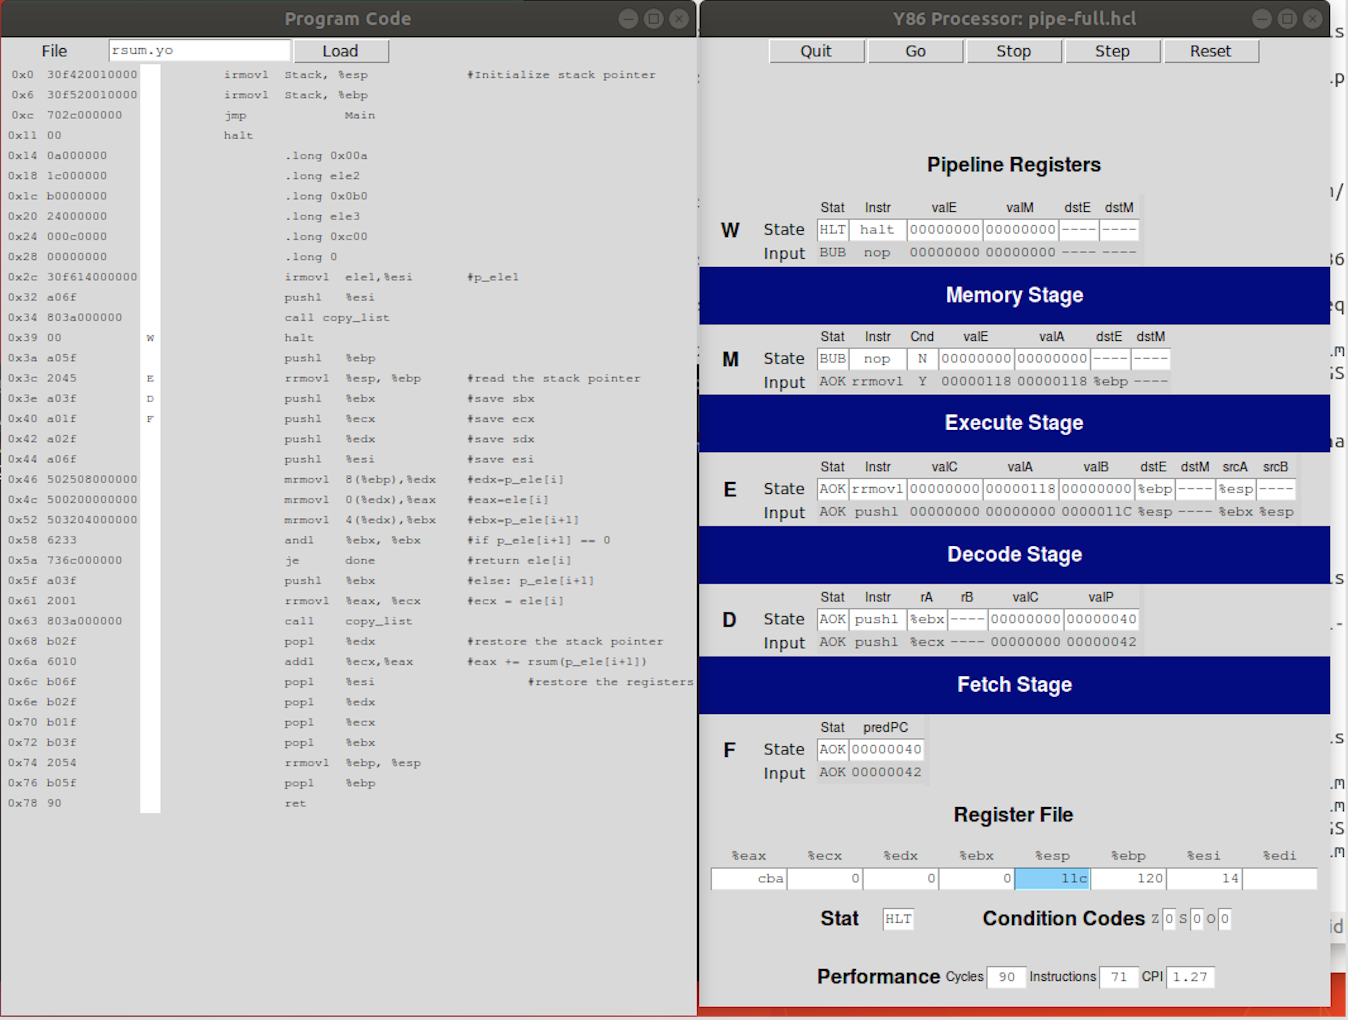
\includegraphics[width=0.95\textwidth]{A-rsum.png}
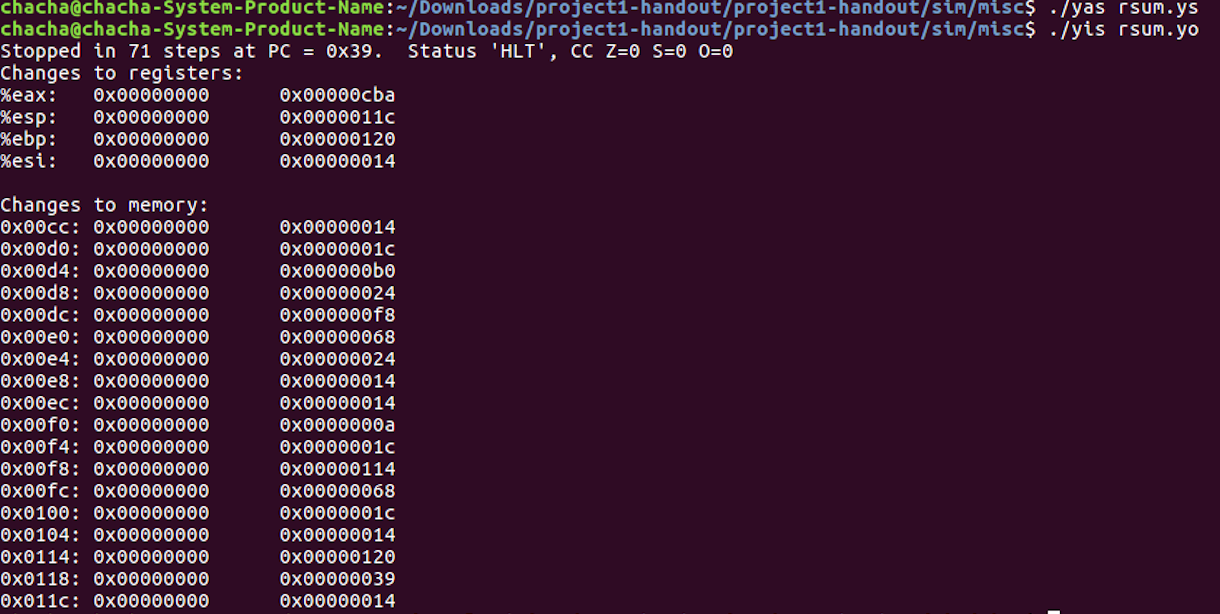
\includegraphics[width=0.95\textwidth]{rsum.png}
As is shown above, our implementation can be seen as successful.

\item \textbf{copy.ys}

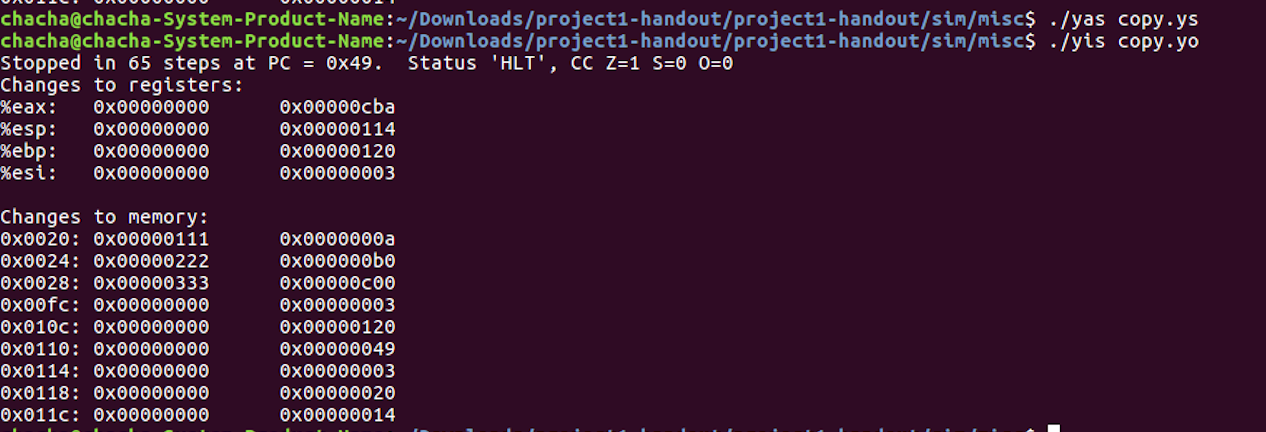
\includegraphics[width=0.95\textwidth]{copy.png}
As is shown above, our implementation can be seen as successful.

\end{itemize}

Target register is returned with correct value and also, from the GUI interface, we could see the performance of CPU as well as the decoded machine language denoted by hexadecimal numbers.

\subsection{Part B}
An operation $iaddl$ added to the control file \textit{seq−full.hcl} to extend the SEQ processor is required in this part. (Also, leave instruction is also implemented although it is not used in our y86 programs so we are not going to details about leave.)
\subsubsection{Analysis}
To add $iaddl$ to the SEQ processor, the steps is as follows:

\begin{enumerate}
\item $M_1[PC]$ is used to get the icode and ifun which combine a byte.
\item  As indicated in the binary code of iaddl, the lower 4 bits of M1[pC+1] are used, so register rB is the register to add with the constant value, while the higher 4 bits of M1[pC+1] is F, indicating rA is not valid. \\
    Then, we get the rest lower 4 bytes of the instruction to get the instant value.
\item Decode the instruction by which we could get the value in the register and store it in the valB.
\item Execute the add operation.
\item Write the result back to the register and Finally update the PC to prepare for the next instruction. The updated PC should be PC+6 since the length of iaddl instruction is designed to be 6 bytes.
\end{enumerate}


\subsubsection{Code}
  \begin{lstlisting}[caption={}]
#/* $begin seq-all-hcl */
####################################################################
#Descriptions:                                                     #
#1.iaddl(6bytes) c0 FrB vv vv vv vv    2.leave(1byte) d0           #
#  result:rB += ConstV                    result:%esp=%ebp+4;      #
#F: icode:ifun<- M1[PC]                          %ebp=M[%ebp]      #
#   rA:rB<-M1[PC+1]                     F: icode:ifun<-M1[PC]      #
#   valC<-M4[PC+2]                         valP<-PC+1              #
#   valP<-PC+6                          D: valA<-R[%esp]           #
#D: valB<-R[rB]                         E: valE<-valA+4            #
#E: valE<-valB+valC                     M: valM<-M[%ebp]           #
#M:                                     WB:R[%esp]<-valE           #
#WB:R[rB]<-valE                            R[%ebp]<-valM           #
####################################################################
#iaddl Details:							   						   #
# iaddl is similar to both addl and irmovl. Actually we can replace#
# this instruction with a combination of irmovl and addl. So we can#
# refer to IIRMOVL and IOPL to implement IIADDL. Here are the 	   #
# the related modifications below.		   #
# 1.instr_vali							   #
# 2.need_regids							   #
# 3.need_valC							   # 
# 4.srcB - rB							   # 
# 5.dstE - rB							   # 
# 6.aluA - valC							   # 
# 7.aluB - valB							   # 
# 8.set_cc							   	   # 
#leave Details:							   # 
# leave is a little more complicated. But by careful analysis, we  #
# can have it implemented with some modifications below.  	   	   #
# 1.instr_vali							   # 
# 2.need_regids							   # 
# 3.srcA - REBP							   # 
# 4.dstE - RESP							   # 
# 5.dstM - REBP							   # 
# 6.aluA - valA							   # 
# 7.aluB - 4							   # 
# 8.mem_read							   # 
# 9.mem_addr - valA						   # 
####################################################################
####################################################################


####################################################################
#    C Include's.  Don't alter these                               #
####################################################################

quote '#include <stdio.h>'
quote '#include "isa.h"'
quote '#include "sim.h"'
quote 'int sim_main(int argc, char *argv[]);'
quote 'int gen_pc(){return 0;}'
quote 'int main(int argc, char *argv[])'
quote '  {plusmode=0;return sim_main(argc,argv);}'

####################################################################
#    Declarations.  Do not change/remove/delete any of these       #
####################################################################

##### Symbolic representation of Y86 Instruction Codes #############
intsig INOP 	'I_NOP'
intsig IHALT	'I_HALT'
intsig IRRMOVL	'I_RRMOVL'
intsig IIRMOVL	'I_IRMOVL'
intsig IRMMOVL	'I_RMMOVL'
intsig IMRMOVL	'I_MRMOVL'
intsig IOPL	'I_ALU'
intsig IJXX	'I_JMP'
intsig ICALL	'I_CALL'
intsig IRET	'I_RET'
intsig IPUSHL	'I_PUSHL'
intsig IPOPL	'I_POPL'
# Instruction code for iaddl instruction
intsig IIADDL	'I_IADDL'
# Instruction code for iaddl instruction
intsig ILEAVE	'I_LEAVE'

##### Symbolic represenations of Y86 function codes                  #####
intsig FNONE    'F_NONE'        # Default function code

##### Symbolic representation of Y86 Registers referenced explicitly #####
intsig RESP     'REG_ESP'    	# Stack Pointer
intsig REBP     'REG_EBP'    	# Frame Pointer
intsig RNONE    'REG_NONE'   	# Special value indicating "no register"

##### ALU Functions referenced explicitly                            #####
intsig ALUADD	'A_ADD'		# ALU should add its arguments

##### Possible instruction status values                             #####
intsig SAOK	'STAT_AOK'		# Normal execution
intsig SADR	'STAT_ADR'	# Invalid memory address
intsig SINS	'STAT_INS'	# Invalid instruction
intsig SHLT	'STAT_HLT'	# Halt instruction encountered

##### Signals that can be referenced by control logic ####################

##### Fetch stage inputs		#####
intsig pc 'pc'				# Program counter
##### Fetch stage computations		#####
intsig imem_icode 'imem_icode'		# icode field from instruction memory
intsig imem_ifun  'imem_ifun' 		# ifun field from instruction memory
intsig icode	  'icode'		# Instruction control code
intsig ifun	  'ifun'		# Instruction function
intsig rA	  'ra'			# rA field from instruction
intsig rB	  'rb'			# rB field from instruction
intsig valC	  'valc'		# Constant from instruction
intsig valP	  'valp'		# Address of following instruction
boolsig imem_error 'imem_error'		# Error signal from instruction memory
boolsig instr_valid 'instr_valid'	# Is fetched instruction valid?

##### Decode stage computations		#####
intsig valA	'vala'			# Value from register A port
intsig valB	'valb'			# Value from register B port

##### Execute stage computations	#####
intsig valE	'vale'			# Value computed by ALU
boolsig Cnd	'cond'			# Branch test

##### Memory stage computations		#####
intsig valM	'valm'			# Value read from memory
boolsig dmem_error 'dmem_error'		# Error signal from data memory


####################################################################
#    Control Signal Definitions.                                   #
####################################################################

################ Fetch Stage     ###################################

# Determine instruction code
int icode = [
	imem_error: INOP;
	1: imem_icode;		# Default: get from instruction memory
];

# Determine instruction function
int ifun = [
	imem_error: FNONE;
	1: imem_ifun;		# Default: get from instruction memory
];

bool instr_valid = icode in
	{ INOP, IHALT, IRRMOVL, IIRMOVL, IRMMOVL, IMRMOVL, IIADDL, ILEAVE,
	       IOPL, IJXX, ICALL, IRET, IPUSHL, IPOPL };

# Does fetched instruction require a regid byte?
bool need_regids =
	icode in { IRRMOVL, IOPL, IPUSHL, IPOPL, IIADDL, ILEAVE,
		     IIRMOVL, IRMMOVL, IMRMOVL };

# Does fetched instruction require a constant word?
bool need_valC =
	icode in { IIRMOVL, IRMMOVL, IMRMOVL, IJXX, ICALL, IIADDL };

################ Decode Stage    ###################################

## What register should be used as the A source?
int srcA = [
	icode in { IRRMOVL, IRMMOVL, IOPL, IPUSHL  } : rA;
	icode in { IPOPL, IRET } : RESP;
	icode in { ILEAVE } : REBP;
	1 : RNONE; # Don't need register
];

## What register should be used as the B source?
int srcB = [
	icode in { IOPL, IRMMOVL, IMRMOVL, IIADDL  } : rB;
	icode in { IPUSHL, IPOPL, ICALL, IRET } : RESP;
	1 : RNONE;  # Don't need register
];

## What register should be used as the E destination?
int dstE = [
	icode in { IRRMOVL } && Cnd : rB;
	icode in { IIRMOVL, IOPL, IIADDL} : rB;
	icode in { IPUSHL, IPOPL, ICALL, IRET, ILEAVE } : RESP;
	1 : RNONE;  # Don't write any register
];

## What register should be used as the M destination?
## Acquire data from memory, and send it to a register
## iaddl doesn't require memory's data
int dstM = [
	icode in { IMRMOVL, IPOPL } : rA;
	icode in { ILEAVE } : REBP;
	1 : RNONE;  # Don't write any register
];

################ Execute Stage   ###################################

## Select input A to ALU
int aluA = [
	icode in { IRRMOVL, IOPL } : valA;
	icode in { IIRMOVL, IRMMOVL, IMRMOVL, IIADDL } : valC;
	icode in { ICALL, IPUSHL } : -4;
	icode in { IRET, IPOPL, ILEAVE } : 4;
	# Other instructions don't need ALU
];

## Select input B to ALU
int aluB = [
	icode in { IRMMOVL, IMRMOVL, IOPL, ICALL,
		      IPUSHL, IRET, IPOPL, IIADDL } : valB;
	icode in { IRRMOVL, IIRMOVL } : 0;
	icode in { ILEAVE } : valA;
	# Other instructions don't need ALU
];

## Set the ALU function
int alufun = [
	icode == IOPL : ifun;
	1 : ALUADD;
];

## Should the condition codes be updated?
bool set_cc = icode in { IOPL, IIADDL };

################ Memory Stage    ###################################

## Set read control signal
bool mem_read = icode in { IMRMOVL, IPOPL, IRET, ILEAVE };

## Set write control signal
bool mem_write = icode in { IRMMOVL, IPUSHL, ICALL };

## Select memory address
int mem_addr = [
	icode in { IRMMOVL, IPUSHL, ICALL, IMRMOVL } : valE;
	icode in { IPOPL, IRET, ILEAVE } : valA;
	# Other instructions don't need address
];

## Select memory input data
int mem_data = [
	# Value from register
	icode in { IRMMOVL, IPUSHL } : valA;
	# Return PC
	icode == ICALL : valP;
	# Default: Don't write anything
];

## Determine instruction status
int Stat = [
	imem_error || dmem_error : SADR;
	!instr_valid: SINS;
	icode == IHALT : SHLT;
	1 : SAOK;
];

################ Program Counter Update ############################

## What address should instruction be fetched at

int new_pc = [
	# Call.  Use instruction constant
	icode == ICALL : valC;
	# Taken branch.  Use instruction constant
	icode == IJXX && Cnd : valC;
	# Completion of RET instruction.  Use value from stack
	icode == IRET : valM;
	# Default: Use incremented PC
	1 : valP;
];
#/* $end seq-all-hcl */


\end{lstlisting}


\subsubsection{Evaluation}

\begin{itemize}
\item Test for $asumi$ \& $asuml$

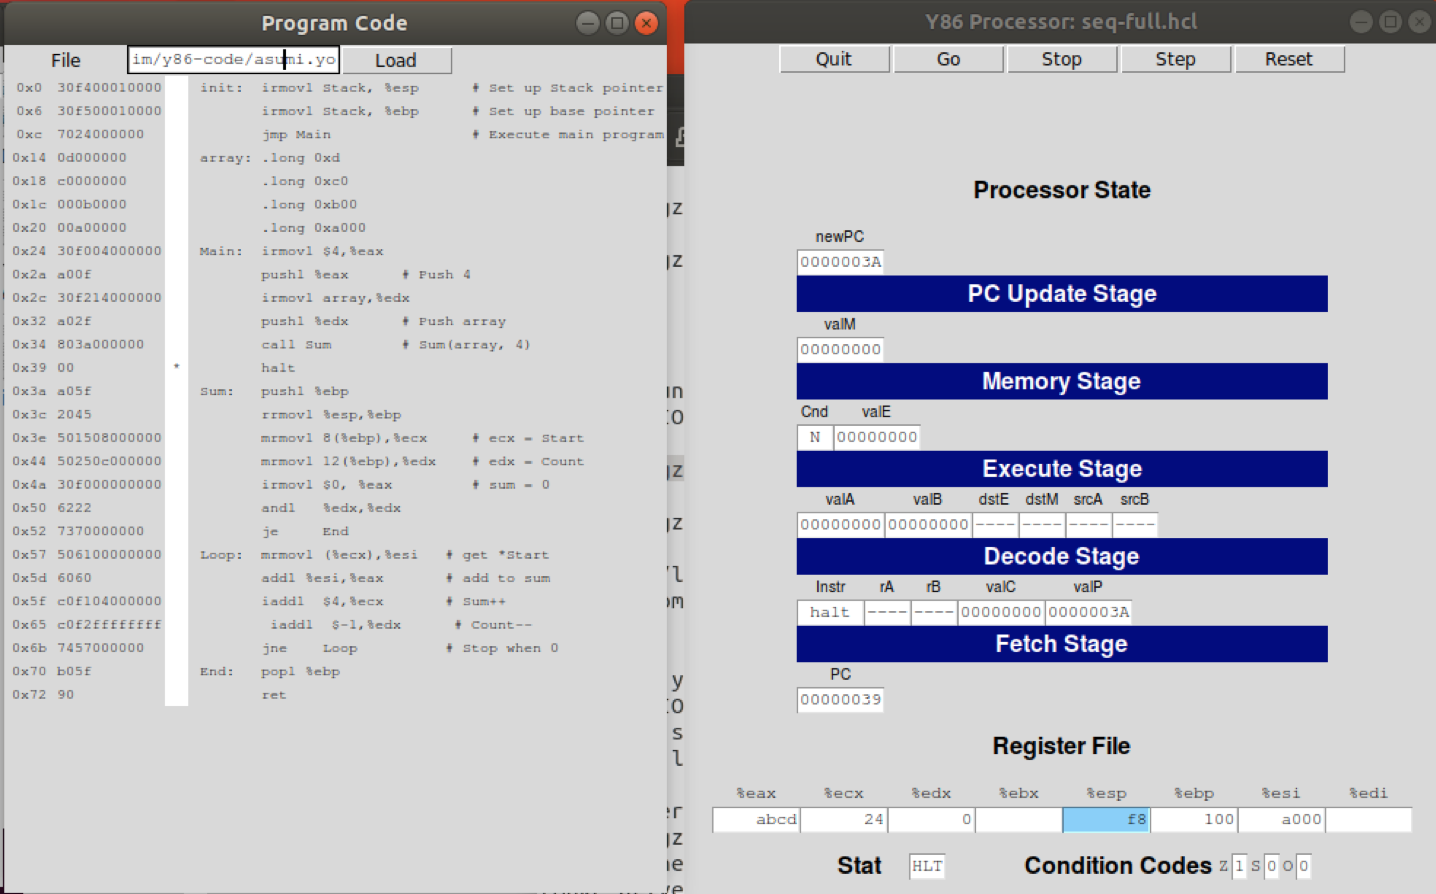
\includegraphics[width=0.95\textwidth]{asumi.png}


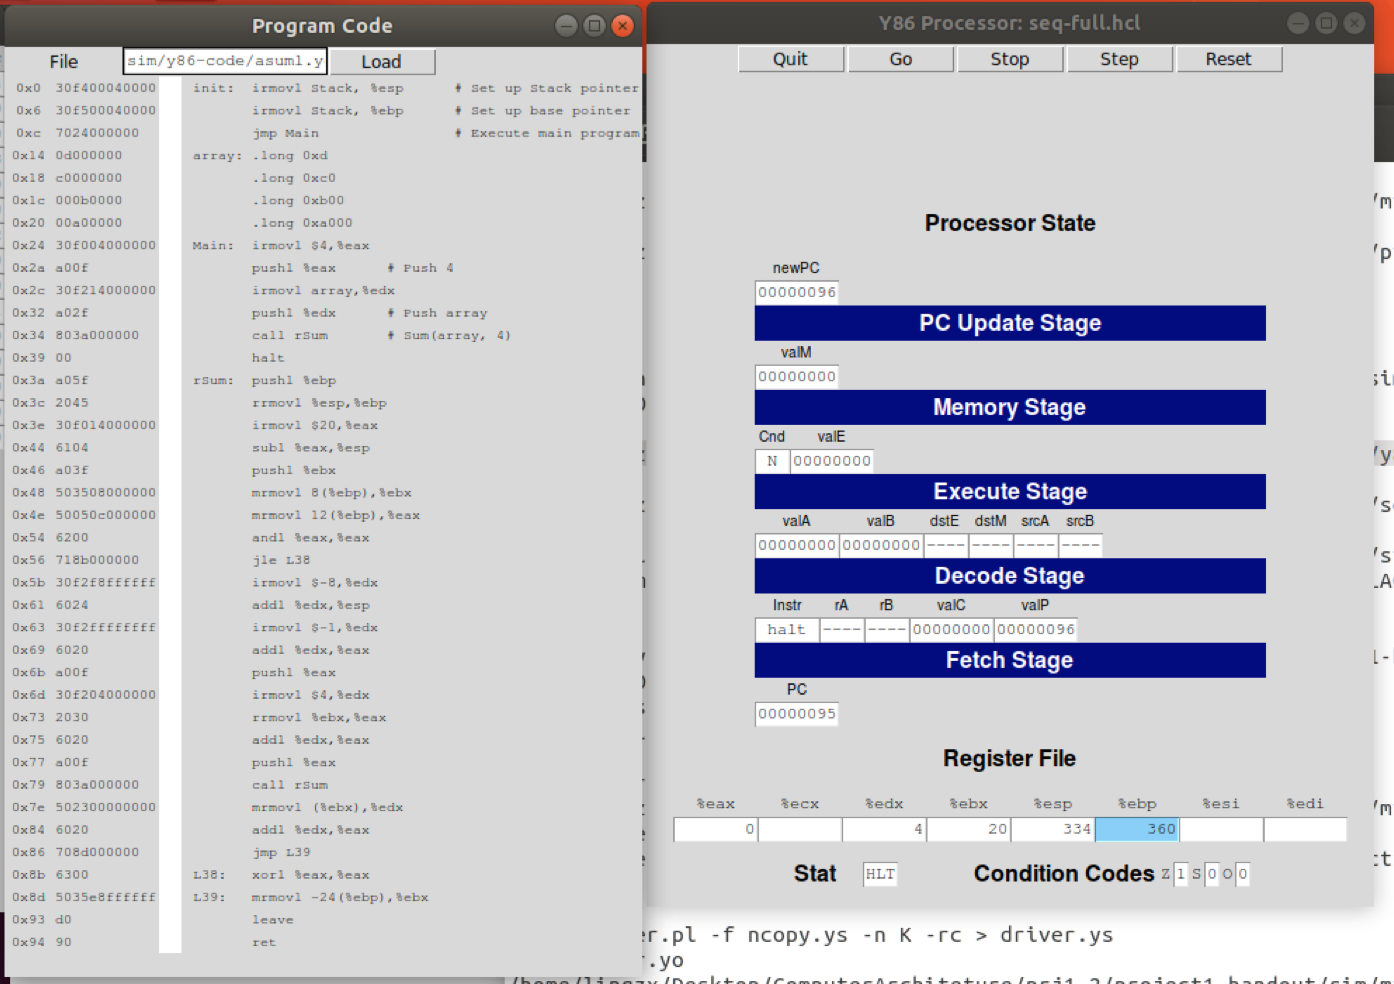
\includegraphics[width=0.95\textwidth]{asuml.png}
\item Retest using the benchmark programs

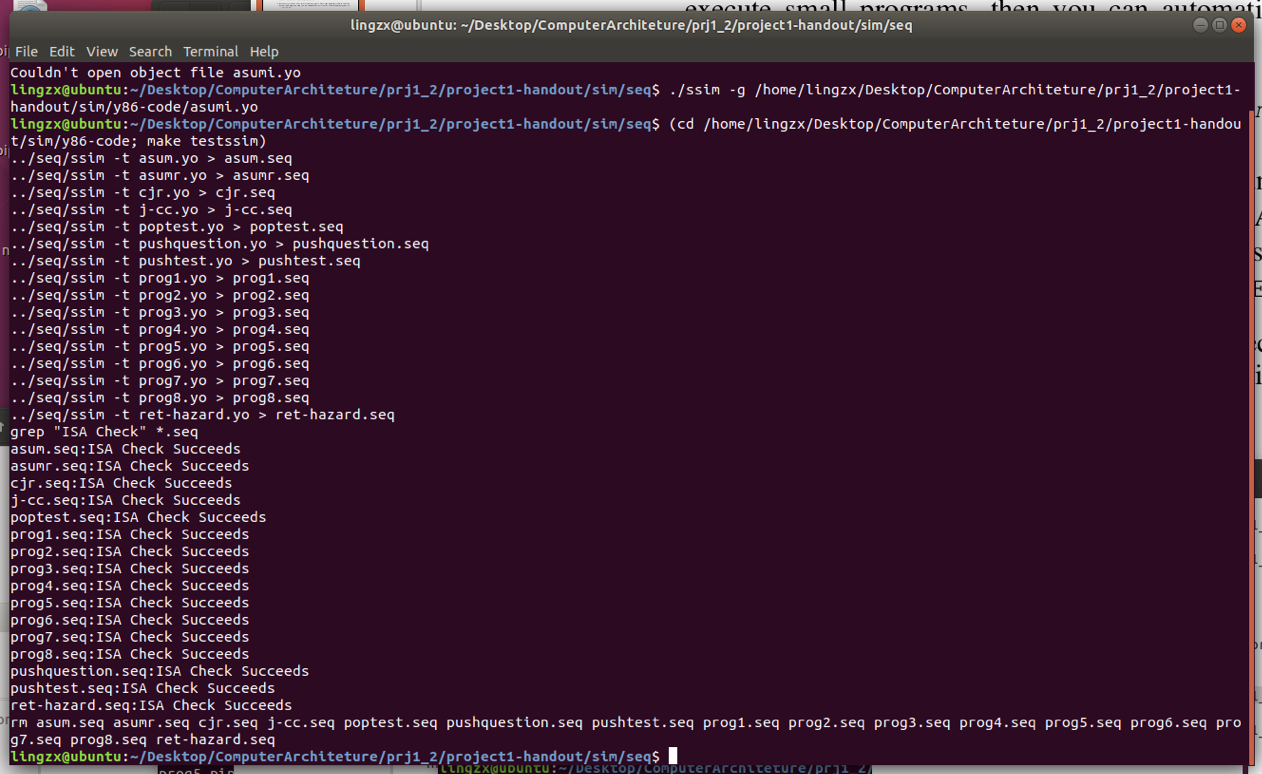
\includegraphics[width=0.95\textwidth]{benchmark.png}

\item Perform regression tests

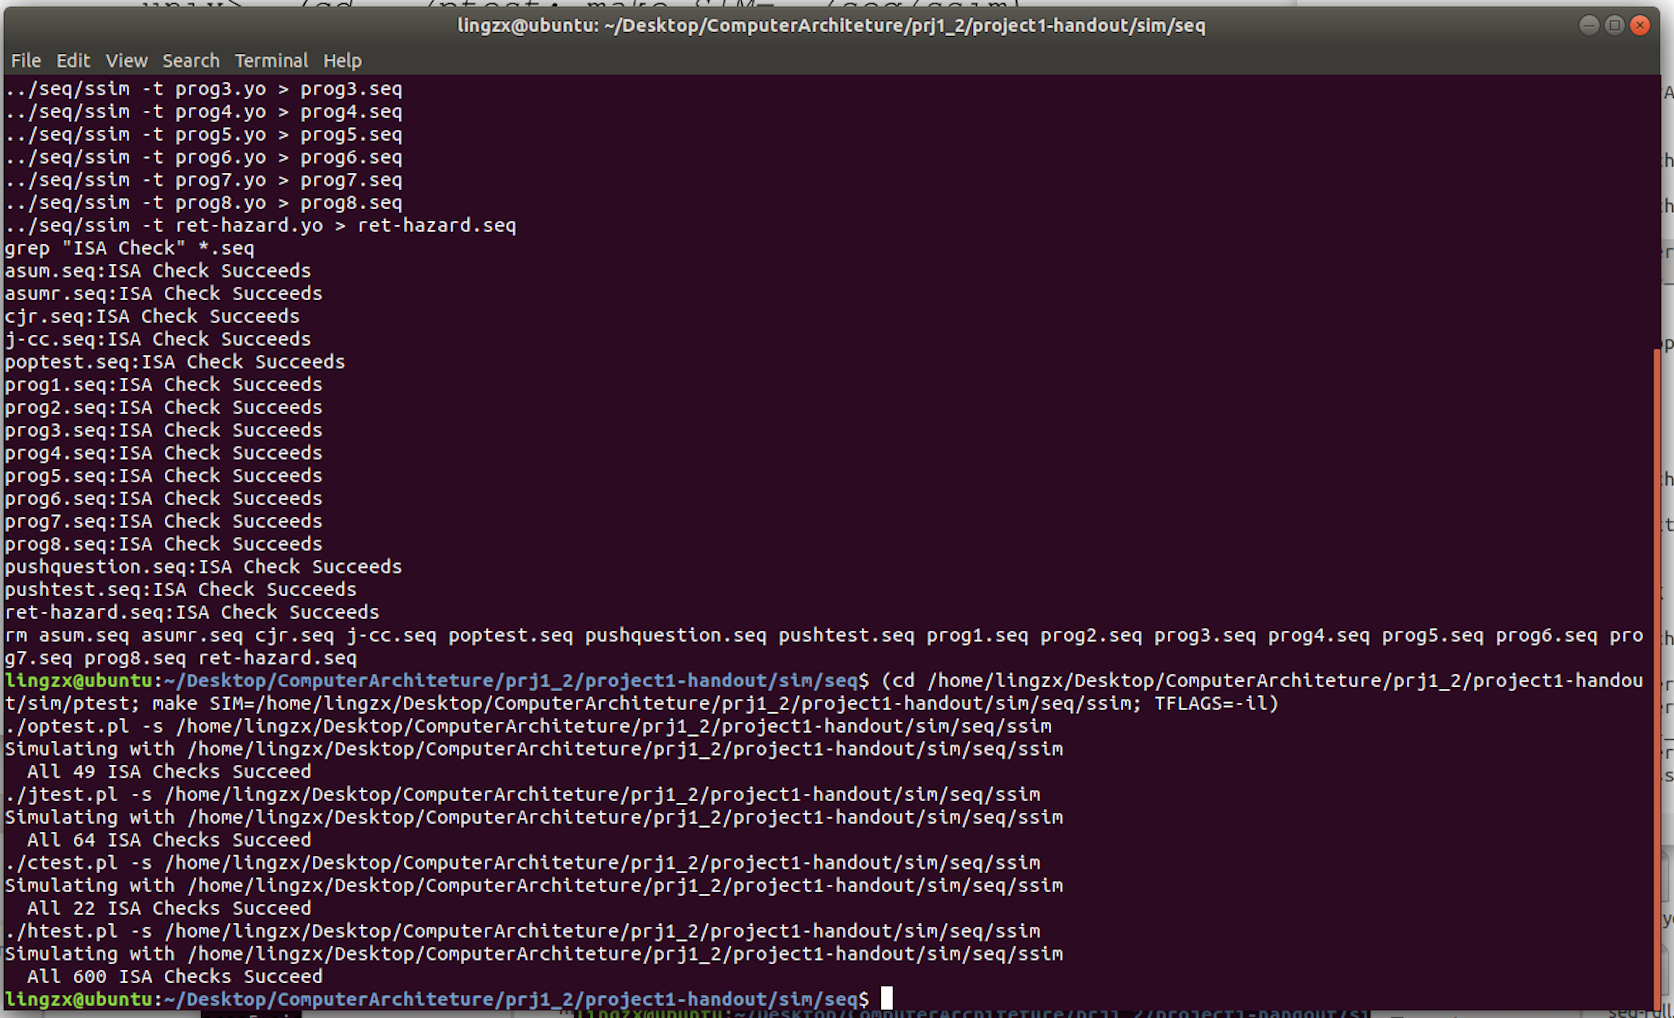
\includegraphics[width=0.95\textwidth]{regressionn.png}

\end{itemize}
\subsection{Part C}

\subsubsection{Analysis}

   \par In this part, we are required to optimize the performance of a function ncopy, which copies the data from source address to destine address and return the number of positive integers contained in the source. And to achieve this goal, optimization of both algorithm and hardware is allowed. So, this part is a test of our overall capability of pipeline architecture.
    \par  The performance of the function is evaluated with CPE, so what we need to do is to reduce average CPE as more as possible. The difficulties lie in several aspects below, and we have also figured out the answer.
\begin{enumerate}
    \item
	What makes the function perform poorly? A: Great number of branch instructions, high cost of computation involving immediate integers and stall penalty from load-read instructions. We are not talking about misprediction penalty of conditional branches but just the proportion of branch instructions that would cost a lot of cycles.
    \item
	How can we reduce branch instructions, computation cost and stall penalty? A: Reduce instructions of conditional branches to improve our algorithm, add new instruction(s) to increase support for immediate computation and adjust sequence of some instructions.
    \item
	What should we do in software layer? A: Modify ncopy.ys, and apply technique of loop unrolling to reduce number of branch instructions, use instruction(s) that supports immediate computation better when necessary and adjust sequence of some instructions that would cause a data hazard.
    \item
	What should we do in hardware layer? A: Modify pipe-full.hcl, and implement logic that supports immediate computation, that is iaddl. (Apart from iaddl, ileave is also implemented here according to the requirement but it is found to be of no use in this part.)
Now we will elaborate what we do here.
\end{enumerate}
	   \par Firstly, loop unrolling. Technique of loop unrolling reduces the number of branch instructions and thus reduce the number of instructions to execute. We have a loop that performs ncopy of 16 elements. In the primitive version of ncopy every time a number is copied there would be a check whether the loop should be over. Thus, we reduce the number of instructions by 15 every 16 elements, which also means that the CPE could be decreased by about 15/16 with technique of loop unrolling. Also, we need to tie up some loose ends. To achieve better performance, after the 16-element loop, we do the ncopy work with 8, 4, 2 and 1 element(s) successively if there are that many elements left.
	   \par Secondly, use iaddl for immediate computation. Decreasing of len and increasing of count, p\_src and p\_dst are involved with immediate operands. We could have CPE decreased by 2 with this step.
	   \par Thirdly, avoid load-read stall penalty. It is easy to find a“mrmovl x1, x2” instruction followed by a “rmmovl x2, x3” instruction, which intends to copy *p\_x1 to *p\_x3. But since mrmovl is a load instruction and rmmovl needs to read the same register. So, codes like this would cause a penalty of one cycle. In other words, by inserting some other instructions into the two instructions can decrease the CPE approximately by 1.
	   \par Fourthly, implementation of iaddl and ileave. Detailed descriptions of iaddl and leave can be seen in the beginning part of seq-full.hcl and pipe-full.hcl. (Although we are talking about implementation of pipeline processor, but the operations of the two instructions are similar to that of a sequence processor) . iaddl, which adds an immediate operand to a register, can be accomplished by combination of irmovl and addl. leave, which decrease stack pointer and load data to base pointer register memory addressed by itself, can be accomplished y combination of mrmovl and popl. Inspired by instructions similar to them, we could modify the hcl file properly. Here are some further details. Iaddl: instr\_vali, need\_regids, need\_valC, d\_srcB = D\_rB, d\_dstE = D\_rB, aluA = valC, aluB = valB, set\_cc. leave: instr\_vali, need\_regids, d\_srcA = REBP, d\_dstE = RESP, d\_dstM = REBP, aluA = E\_valA, aluB = 4, mem\_addr = M\_valA, mem\_read, F\_stall, D\_stall, D\_bubble, E\_bubble. Using iaddl instruction can also reduce CPE by about 2.\\


\subsubsection{Code}

\begin{itemize}
\item \textbf{ncopy.ys}
  \begin{lstlisting}[caption={}]
#/* $begin ncopy-ys */
# 948bytes < 1000bytes
# Average CPE = 9.89
# The trick used in the ncopy function is loop unrolling.
# 1.Fisrt we iteratively 'ncopy' 16 elements until there are fewer 
# than 16 elements left.
# 2.Then check if left elements are more than 8, and if so,
# we 'ncopy' 8 elements.
# 3.Repeat procedure2 by checking and 'ncopy' 4, 2, 1 element(s).
# The modifications above reduces number of condition branch 
# instructions, and thus improve the performance of CPU. 
# Also, some sequences of instructions are modified.
# Src-plus and count-plus instructions are inserted between
# some mrmovl and rmmovl instructions to avoid a stalling
# due to data hazard.
######################################################
# ncopy.ys - Copy a src block of len ints to dst.
# Return the number of positive ints (>0) contained in src.
#
# Include your name and ID here.
#
# Describe how and why you modified the baseline code.
#
######################################################
# Do not modify this portion
# Function prologue.
ncopy:	pushl %ebp		# Save old frame pointer
	rrmovl %esp,%ebp	# Set up new frame pointer
	pushl %esi		# Save callee-save regs
	pushl %ebx
	pushl %edi
	mrmovl 8(%ebp),%ebx	# src
	mrmovl 16(%ebp),%edx	# len
	mrmovl 12(%ebp),%ecx	# dst

######################################################
# You can modify this portion
xorl %eax,%eax		# count = 0;

############## Iteratively 'ncopy' 16 elements until #############
############## fewer than 16 elements left. 	     #############		
Loop5:	iaddl  $-16,%edx	# len-=16 > 0 ?
	jl Loop4		# if so, goto Loop:

	mrmovl (%ebx), %esi	# read val from src...
	andl %esi, %esi		# val <= 0?
	jle Npos51		# if so, goto Npos:
	iaddl  $1, %eax		# count++
Npos51:	rmmovl %esi, (%ecx)	# ...and store it to dst

	mrmovl 4(%ebx), %esi	# read val from src...
	andl %esi, %esi		# val <= 0?
	jle Npos52		# if so, goto Npos:
	iaddl  $1, %eax		# count++
Npos52:	rmmovl %esi, 4(%ecx)	# ...and store it to dst

	mrmovl 8(%ebx), %esi	# read val from src...
	andl %esi, %esi		# val <= 0?
	jle Npos53		# if so, goto Npos:
	iaddl  $1, %eax		# count++
Npos53:	rmmovl %esi, 8(%ecx)	# ...and store it to dst

	mrmovl 12(%ebx), %esi	# read val from src...
	andl %esi, %esi		# val <= 0?
	jle Npos54		# if so, goto Npos:
	iaddl  $1, %eax		# count++
Npos54:	rmmovl %esi, 12(%ecx)	# ...and store it to dst

	mrmovl 16(%ebx), %esi	# read val from src...
	andl %esi, %esi		# val <= 0?
	jle Npos55		# if so, goto Npos:
	iaddl  $1, %eax		# count++
Npos55:	rmmovl %esi, 16(%ecx)	# ...and store it to dst

	mrmovl 20(%ebx), %esi	# read val from src...
	andl %esi, %esi		# val <= 0?
	jle Npos56		# if so, goto Npos:
	iaddl  $1, %eax		# count++
Npos56:	rmmovl %esi, 20(%ecx)	# ...and store it to dst

	mrmovl 24(%ebx), %esi	# read val from src...
	andl %esi, %esi		# val <= 0?
	jle Npos57		# if so, goto Npos:
	iaddl  $1, %eax		# count++
Npos57:	rmmovl %esi, 24(%ecx)	# ...and store it to dst

	mrmovl 28(%ebx), %esi	# read val from src...
	andl %esi, %esi		# val <= 0?
	jle Npos58		# if so, goto Npos:
	iaddl  $1, %eax		# count++
Npos58:	rmmovl %esi, 28(%ecx)	# ...and store it to dst

	mrmovl 32(%ebx), %esi	# read val from src...
	andl %esi, %esi		# val <= 0?
	jle Npos59		# if so, goto Npos:
	iaddl  $1, %eax		# count++
Npos59:	rmmovl %esi, 32(%ecx)	# ...and store it to dst

	mrmovl 36(%ebx), %esi	# read val from src...
	andl %esi, %esi		# val <= 0?
	jle Npos510		# if so, goto Npos:
	iaddl  $1, %eax		# count++
Npos510:rmmovl %esi, 36(%ecx)	# ...and store it to dst

	mrmovl 40(%ebx), %esi	# read val from src...
	andl %esi, %esi		# val <= 0?
	jle Npos511		# if so, goto Npos:
	iaddl  $1, %eax		# count++
Npos511:rmmovl %esi, 40(%ecx)	# ...and store it to dst

	mrmovl 44(%ebx), %esi	# read val from src...
	andl %esi, %esi		# val <= 0?
	jle Npos512		# if so, goto Npos:
	iaddl  $1, %eax		# count++
Npos512:rmmovl %esi, 44(%ecx)	# ...and store it to dst

	mrmovl 48(%ebx), %esi	# read val from src...
	andl %esi, %esi		# val <= 0?
	jle Npos513		# if so, goto Npos:
	iaddl  $1, %eax		# count++
Npos513:rmmovl %esi, 48(%ecx)	# ...and store it to dst

	mrmovl 52(%ebx), %esi	# read val from src...
	andl %esi, %esi		# val <= 0?
	jle Npos514		# if so, goto Npos:
	iaddl  $1, %eax		# count++
Npos514:rmmovl %esi, 52(%ecx)	# ...and store it to dst

	mrmovl 56(%ebx), %esi	# read val from src...
	andl %esi, %esi		# val <= 0?
	jle Npos515		# if so, goto Npos:
	iaddl  $1, %eax		# count++
Npos515:rmmovl %esi, 56(%ecx)	# ...and store it to dst

	mrmovl 60(%ebx), %esi	# read val from src...
	iaddl  $64,%ebx		# src+=16
	rmmovl %esi, 60(%ecx)	# ...and store it to dst
	andl %esi, %esi		# val <= 0?
	jle Npos516		# if so, goto Npos:
	iaddl  $1, %eax		# count++
Npos516:iaddl  $64,%ecx		# dst+=16
	jmp Loop5		# goto Loop:
########## Iterative 'ncopy' of 16 elements is over ###########



### Check if left elements are more than 8, and if so, ########
### we 'ncopy' 8 elements.			###############
Loop4:	iaddl  $8,%edx		# len-=4 > 0 ?
	jl Loop3		# if so, goto Loop:

	mrmovl (%ebx), %esi	# read val from src...
	andl %esi, %esi		# val <= 0?
	jle Npos41		# if so, goto Npos:
	iaddl  $1, %eax		# count++
Npos41:	rmmovl %esi, (%ecx)	# ...and store it to dst

	mrmovl 4(%ebx), %esi	# read val from src...
	andl %esi, %esi		# val <= 0?
	jle Npos42		# if so, goto Npos:
	iaddl  $1, %eax		# count++
Npos42:	rmmovl %esi, 4(%ecx)	# ...and store it to dst

	mrmovl 8(%ebx), %esi	# read val from src...
	andl %esi, %esi		# val <= 0?
	jle Npos43		# if so, goto Npos:
	iaddl  $1, %eax		# count++
Npos43:	rmmovl %esi, 8(%ecx)	# ...and store it to dst

	mrmovl 12(%ebx), %esi	# read val from src...
	andl %esi, %esi		# val <= 0?
	jle Npos44		# if so, goto Npos:
	iaddl  $1, %eax		# count++
Npos44:	rmmovl %esi, 12(%ecx)	# ...and store it to dst

	mrmovl 16(%ebx), %esi	# read val from src...
	andl %esi, %esi		# val <= 0?
	jle Npos45		# if so, goto Npos:
	iaddl  $1, %eax		# count++
Npos45:	rmmovl %esi, 16(%ecx)	# ...and store it to dst

	mrmovl 20(%ebx), %esi	# read val from src...
	andl %esi, %esi		# val <= 0?
	jle Npos46		# if so, goto Npos:
	iaddl  $1, %eax		# count++
Npos46:	rmmovl %esi, 20(%ecx)	# ...and store it to dst

	mrmovl 24(%ebx), %esi	# read val from src...
	andl %esi, %esi		# val <= 0?
	jle Npos47		# if so, goto Npos:
	iaddl  $1, %eax		# count++
Npos47:	rmmovl %esi, 24(%ecx)	# ...and store it to dst

	mrmovl 28(%ebx), %esi	# read val from src...
	iaddl  $32,%ebx		# src+=8
	rmmovl %esi, 28(%ecx)	# ...and store it to dst
	andl %esi, %esi		# val <= 0?
	jle Npos48		# if so, goto Npos:
	iaddl  $1, %eax		# count++
Npos48:	iaddl  $32,%ecx		# dst+=8
	iaddl  $-8,%edx
######### End of 8-element checking and 'ncopy ##########


### Check if left elements are more than 4, and if so, ########
### we 'ncopy' 4 elements.			###############
Loop3:	iaddl  $4,%edx		# len-=4 > 0 ?
	jl Loop2		# if so, goto Loop:

	mrmovl (%ebx), %esi	# read val from src...
	andl %esi, %esi		# val <= 0?
	jle Npos31		# if so, goto Npos:
	iaddl  $1, %eax		# count++
Npos31:	rmmovl %esi, (%ecx)	# ...and store it to dst

	mrmovl 4(%ebx), %esi	# read val from src...
	andl %esi, %esi		# val <= 0?
	jle Npos32		# if so, goto Npos:
	iaddl  $1, %eax		# count++
Npos32:	rmmovl %esi, 4(%ecx)	# ...and store it to dst

	mrmovl 8(%ebx), %esi	# read val from src...
	andl %esi, %esi		# val <= 0?
	jle Npos33		# if so, goto Npos:
	iaddl  $1, %eax		# count++
Npos33:	rmmovl %esi, 8(%ecx)	# ...and store it to dst

	mrmovl 12(%ebx), %esi	# read val from src...
	iaddl  $16,%ebx		# src++++++++
	rmmovl %esi, 12(%ecx)	# ...and store it to dst
	andl %esi, %esi		# val <= 0?
	jle Npos34		# if so, goto Npos:
	iaddl  $1, %eax		# count++
Npos34:	iaddl  $16,%ecx		# dst++++++++
	iaddl  $-4,%edx
######### End of 4-element checking and 'ncopy ##########


### Check if left elements are more than 2, and if so, ########
### we 'ncopy' 2 elements.			###############
Loop2:	iaddl  $2,%edx		# len+2 < 0 ?
	jl Loop1		# if so, goto Loop1:
	mrmovl (%ebx), %esi	# read val from src...
	andl %esi, %esi		# val <= 0?
	jle Npos21		# if so, goto Npos:
	iaddl  $1, %eax		# count++
Npos21:	rmmovl %esi, (%ecx)	# ...and store it to dst
	mrmovl 4(%ebx), %esi	# read val from src...
	iaddl  $8,%ebx		# src++++
	rmmovl %esi, 4(%ecx)	# ...and store it to dst
	andl %esi, %esi		# val <= 0?
	jle Npos22		# if so, goto Npos:
	iaddl  $1, %eax		# count++
Npos22:	iaddl  $8, %ecx		# dst++++
	iaddl  $-2,%edx
######### End of 2-element checking and 'ncopy ##########


### Check if left elements are more than 1, and if so, ########
### we 'ncopy' 1 elements.			###############
Loop1:  iaddl $1,%edx		# len+1 < 0?
	jl Done			# if so, goto Done:
	mrmovl (%ebx), %esi	# read val from src...
	iaddl  $4,%ebx		# src++
	rmmovl %esi, (%ecx)	# ...and store it to dst
	andl %esi, %esi		# val <= 0?
	jle Done		# if so, goto Npos:
	iaddl  $1, %eax		# count++
######### End of 1-element checking and 'ncopy ##########

# Do not modify the following section of code
# Function epilogue.
Done:
	popl %edi               # Restore callee-save registers
	popl %ebx
	popl %esi
	rrmovl %ebp, %esp
	popl %ebp
	ret
######################################################
# Keep the following label at the end of your function
End:
#/* $end ncopy-ys */

   \end{lstlisting}


\item \textbf{pipe-full.hcl}
  \begin{lstlisting}[caption={}]
#/* $begin pipe-all-hcl */
######################################################
#    HCL Description of Control for Pipelined Y86 Processor        #
#    Copyright (C) Randal E. Bryant, David R. O'Hallaron, 2010     #
######################################################

## Your task is to implement the iaddl and leave instructions
## The file contains a declaration of the icodes
## for iaddl (IIADDL) and leave (ILEAVE).
## Your job is to add the rest of the logic to make it work

######################################################
######################################################
#                   Leader's name and ID.                          #
######################################################
#Descriptions:							   #
# Both instructions leave and iaddl are implemented here, which are#
# similar to those of 'seq'.					   #
# For iaddl/IIADDL, the work is almost the same as that of 'seq'   #
# version. The difference is that information, such as source	   #
# register or destine register is acquired from pipeline registers.#
# (It's very lucky to see all forwarding logic has already been    #
# implmeneted)							   #
# For leave/ILEAVE, the work is more complicated. Since this is a  #
# load instruction, attention must be paid to avoidance of data    #
# hazards. By careful analysis, we decide that ILEAVE can be 	   #
# grouped with IMRMOVL, IPOPL when coping with data hazards, which #
# largely reduced complexity of the job.			   #
######################################################
#iaddl Details:							   #
# 1.instr_valid							   #
# 2.need_regids							   #
# 3.need_valC							   #
# 4.d_srcB - D_rB						   #
# 5.d_dstE - D_rB						   #
# 6.aluA - valC							   #
# 7.aluB - valB							   #
# 8.set_cc							   #
#leave Details:							   # 
# 1.instr_vali							   #
# 2.need_regids							   #
# 3.d_srcA - REBP						   #
# 4.d_dstE - RESP						   #
# 5.d_dstM - REBP						   #
# 6.aluA - E_valA						   #
# 7.aluB - 4							   #
# 8.mem_addr - M_valA						   #
# 9.mem_read							   #
# 10.F_stall							   #
# 11.D_stall							   #
# 12.D_bubble							   #
# 13.E_bubble							   #
######################################################
######################################################

######################################################
#    C Include's.  Don't alter these                               #
######################################################

quote '#include <stdio.h>'
quote '#include "isa.h"'
quote '#include "pipeline.h"'
quote '#include "stages.h"'
quote '#include "sim.h"'
quote 'int sim_main(int argc, char *argv[]);'
quote 'int main(int argc, char *argv[]){return sim_main(argc,argv);}'

######################################################
#    Declarations.  Do not change/remove/delete any of these       #
######################################################

##### Symbolic representation of Y86 Instruction Codes #############
intsig INOP 	'I_NOP'
intsig IHALT	'I_HALT'
intsig IRRMOVL	'I_RRMOVL'
intsig IIRMOVL	'I_IRMOVL'
intsig IRMMOVL	'I_RMMOVL'
intsig IMRMOVL	'I_MRMOVL'
intsig IOPL	'I_ALU'
intsig IJXX	'I_JMP'
intsig ICALL	'I_CALL'
intsig IRET	'I_RET'
intsig IPUSHL	'I_PUSHL'
intsig IPOPL	'I_POPL'
# Instruction code for iaddl instruction
intsig IIADDL	'I_IADDL'
# Instruction code for leave instruction
intsig ILEAVE	'I_LEAVE'

##### Symbolic represenations of Y86 function codes            #####
intsig FNONE    'F_NONE'        # Default function code

##### Symbolic representation of Y86 Registers referenced      #####
intsig RESP     'REG_ESP'    	     # Stack Pointer
intsig REBP     'REG_EBP'    	     # Frame Pointer
intsig RNONE    'REG_NONE'   	     # Special value indicating "no register"

##### ALU Functions referenced explicitly ##########################
intsig ALUADD	'A_ADD'		     # ALU should add its arguments

##### Possible instruction status values                       #####
intsig SBUB	'STAT_BUB'	# Bubble in stage
intsig SAOK	'STAT_AOK'	# Normal execution
intsig SADR	'STAT_ADR'	# Invalid memory address
intsig SINS	'STAT_INS'	# Invalid instruction
intsig SHLT	'STAT_HLT'	# Halt instruction encountered

##### Signals that can be referenced by control logic ##############

##### Pipeline Register F ##########################################

intsig F_predPC 'pc_curr->pc'	     # Predicted value of PC

##### Intermediate Values in Fetch Stage ###########################

intsig imem_icode  'imem_icode'      # icode field from instruction memory
intsig imem_ifun   'imem_ifun'       # ifun  field from instruction memory
intsig f_icode	'if_id_next->icode'  # (Possibly modified) instruction code
intsig f_ifun	'if_id_next->ifun'   # Fetched instruction function
intsig f_valC	'if_id_next->valc'   # Constant data of fetched instruction
intsig f_valP	'if_id_next->valp'   # Address of following instruction
boolsig imem_error 'imem_error'	     # Error signal from instruction memory
boolsig instr_valid 'instr_valid'    # Is fetched instruction valid?

##### Pipeline Register D ##########################################
intsig D_icode 'if_id_curr->icode'   # Instruction code
intsig D_rA 'if_id_curr->ra'	     # rA field from instruction
intsig D_rB 'if_id_curr->rb'	     # rB field from instruction
intsig D_valP 'if_id_curr->valp'     # Incremented PC

##### Intermediate Values in Decode Stage  #########################

intsig d_srcA	 'id_ex_next->srca'  # srcA from decoded instruction
intsig d_srcB	 'id_ex_next->srcb'  # srcB from decoded instruction
intsig d_rvalA 'd_regvala'	     # valA read from register file
intsig d_rvalB 'd_regvalb'	     # valB read from register file

##### Pipeline Register E ##########################################
intsig E_icode 'id_ex_curr->icode'   # Instruction code
intsig E_ifun  'id_ex_curr->ifun'    # Instruction function
intsig E_valC  'id_ex_curr->valc'    # Constant data
intsig E_srcA  'id_ex_curr->srca'    # Source A register ID
intsig E_valA  'id_ex_curr->vala'    # Source A value
intsig E_srcB  'id_ex_curr->srcb'    # Source B register ID
intsig E_valB  'id_ex_curr->valb'    # Source B value
intsig E_dstE 'id_ex_curr->deste'    # Destination E register ID
intsig E_dstM 'id_ex_curr->destm'    # Destination M register ID

##### Intermediate Values in Execute Stage #########################
intsig e_valE 'ex_mem_next->vale'	# valE generated by ALU
boolsig e_Cnd 'ex_mem_next->takebranch' # Does condition hold?
intsig e_dstE 'ex_mem_next->deste'      # dstE (possibly modified to be RNONE)

##### Pipeline Register M                  #########################
intsig M_stat 'ex_mem_curr->status'     # Instruction status
intsig M_icode 'ex_mem_curr->icode'	# Instruction code
intsig M_ifun  'ex_mem_curr->ifun'	# Instruction function
intsig M_valA  'ex_mem_curr->vala'      # Source A value
intsig M_dstE 'ex_mem_curr->deste'	# Destination E register ID
intsig M_valE  'ex_mem_curr->vale'      # ALU E value
intsig M_dstM 'ex_mem_curr->destm'	# Destination M register ID
boolsig M_Cnd 'ex_mem_curr->takebranch'	# Condition flag
boolsig dmem_error 'dmem_error'	        # Error signal from instruction memory

##### Intermediate Values in Memory Stage ##########################
intsig m_valM 'mem_wb_next->valm'	# valM generated by memory
intsig m_stat 'mem_wb_next->status'	# stat (possibly modified to be SADR)

##### Pipeline Register W ##########################################
intsig W_stat 'mem_wb_curr->status'     # Instruction status
intsig W_icode 'mem_wb_curr->icode'	# Instruction code
intsig W_dstE 'mem_wb_curr->deste'	# Destination E register ID
intsig W_valE  'mem_wb_curr->vale'      # ALU E value
intsig W_dstM 'mem_wb_curr->destm'	# Destination M register ID
intsig W_valM  'mem_wb_curr->valm'	# Memory M value

###############################################################
#    Control Signal Definitions.                                   #
###############################################################

################ Fetch Stage     ###################################

## What address should instruction be fetched at
int f_pc = [
	# Mispredicted branch.  Fetch at incremented PC
	M_icode == IJXX && !M_Cnd : M_valA;
	# Completion of RET instruction.
	W_icode == IRET : W_valM;
	# Default: Use predicted value of PC
	1 : F_predPC;
];

## Determine icode of fetched instruction
int f_icode = [
	imem_error : INOP;
	1: imem_icode;
];

# Determine ifun
int f_ifun = [
	imem_error : FNONE;
	1: imem_ifun;
];

# Is instruction valid?
bool instr_valid = f_icode in
	{ INOP, IHALT, IRRMOVL, IIRMOVL, IRMMOVL, IMRMOVL, IIADDL, ILEAVE,
	  IOPL, IJXX, ICALL, IRET, IPUSHL, IPOPL };

# Determine status code for fetched instruction
int f_stat = [
	imem_error: SADR;
	!instr_valid : SINS;
	f_icode == IHALT : SHLT;
	1 : SAOK;
];

# Does fetched instruction require a regid byte?
bool need_regids =
	f_icode in { IRRMOVL, IOPL, IPUSHL, IPOPL, IIADDL, ILEAVE,
		     IIRMOVL, IRMMOVL, IMRMOVL };

# Does fetched instruction require a constant word?
bool need_valC =
	f_icode in { IIRMOVL, IRMMOVL, IMRMOVL, IJXX, ICALL, IIADDL };

# Predict next value of PC
int f_predPC = [
	f_icode in { IJXX, ICALL } : f_valC;
	1 : f_valP;
];

################ Decode Stage #################################


## What register should be used as the A source?
int d_srcA = [
	D_icode in { IRRMOVL, IRMMOVL, IOPL, IPUSHL  } : D_rA;
	D_icode in { IPOPL, IRET } : RESP;
	D_icode in { ILEAVE } : REBP;
	1 : RNONE; # Don't need register
];

## What register should be used as the B source?
int d_srcB = [
	D_icode in { IOPL, IRMMOVL, IMRMOVL, IIADDL  } : D_rB;
	D_icode in { IPUSHL, IPOPL, ICALL, IRET } : RESP;
	1 : RNONE;  # Don't need register
];

## What register should be used as the E destination?
int d_dstE = [
	D_icode in { IRRMOVL, IIRMOVL, IOPL, IIADDL} : D_rB;
	D_icode in { IPUSHL, IPOPL, ICALL, IRET, ILEAVE } : RESP;
	1 : RNONE;  # Don't write any register
];

## What register should be used as the M destination?
int d_dstM = [
	D_icode in { IMRMOVL, IPOPL } : D_rA;
	D_icode in { ILEAVE } : REBP;
	1 : RNONE;  # Don't write any register
];

## What should be the A value?
## Forward into decode stage for valA
int d_valA = [
	D_icode in { ICALL, IJXX } : D_valP; # Use incremented PC
	d_srcA == e_dstE : e_valE;    # Forward valE from execute
	d_srcA == M_dstM : m_valM;    # Forward valM from memory
	d_srcA == M_dstE : M_valE;    # Forward valE from memory
	d_srcA == W_dstM : W_valM;    # Forward valM from write back
	d_srcA == W_dstE : W_valE;    # Forward valE from write back
	1 : d_rvalA;  # Use value read from register file
];

int d_valB = [
	d_srcB == e_dstE : e_valE;    # Forward valE from execute
	d_srcB == M_dstM : m_valM;    # Forward valM from memory
	d_srcB == M_dstE : M_valE;    # Forward valE from memory
	d_srcB == W_dstM : W_valM;    # Forward valM from write back
	d_srcB == W_dstE : W_valE;    # Forward valE from write back
	1 : d_rvalB;  # Use value read from register file
];

################ Execute Stage ################################

## Select input A to ALU
int aluA = [
	E_icode in { IRRMOVL, IOPL, ILEAVE } : E_valA;
	E_icode in { IIRMOVL, IRMMOVL, IMRMOVL, IIADDL } : E_valC;
	E_icode in { ICALL, IPUSHL } : -4;
	E_icode in { IRET, IPOPL } : 4;
	# Other instructions don't need ALU
];

## Select input B to ALU
int aluB = [
	E_icode in { IRMMOVL, IMRMOVL, IOPL, ICALL,
		     IPUSHL, IRET, IPOPL, IIADDL } : E_valB;
	E_icode in { IRRMOVL, IIRMOVL } : 0;
	E_icode in { ILEAVE } : 4;
	# Other instructions don't need ALU
];

## Set the ALU function
int alufun = [
	E_icode == IOPL : E_ifun;
	1 : ALUADD;
];

## Should the condition codes be updated?
bool set_cc = (E_icode in {IOPL, IIADDL } ) &&
	# State changes only during normal operation
	!m_stat in { SADR, SINS, SHLT } && !W_stat in { SADR, SINS, SHLT };

## Generate valA in execute stage
int e_valA = E_valA;    # Pass valA through stage

## Set dstE to RNONE in event of not-taken conditional move
int e_dstE = [
	E_icode == IRRMOVL && !e_Cnd : RNONE;
	1 : E_dstE;
];

################ Memory Stage #################################

## Select memory address
int mem_addr = [
	M_icode in { IRMMOVL, IPUSHL, ICALL, IMRMOVL } : M_valE;
	M_icode in { IPOPL, IRET } : M_valA;
	M_icode in { ILEAVE } : M_valA;
	# Other instructions don't need address
];

## Set read control signal
bool mem_read = M_icode in { IMRMOVL, IPOPL, IRET, ILEAVE };

## Set write control signal
bool mem_write = M_icode in { IRMMOVL, IPUSHL, ICALL };

#/* $begin pipe-m_stat-hcl */
## Update the status
int m_stat = [
	dmem_error : SADR;
	1 : M_stat;
];
#/* $end pipe-m_stat-hcl */

## Set E port register ID
int w_dstE = W_dstE;

## Set E port value
int w_valE = W_valE;

## Set M port register ID
int w_dstM = W_dstM;

## Set M port value
int w_valM = W_valM;

## Update processor status
int Stat = [
	W_stat == SBUB : SAOK;
	1 : W_stat;
];

################ Pipeline Register Control ####################

# Should I stall or inject a bubble into Pipeline Register F?
# At most one of these can be true.
bool F_bubble = 0;
bool F_stall =
	# Conditions for a load/use hazard
	E_icode in { IMRMOVL, IPOPL, ILEAVE } &&    #Dst value generated after M stage
	 E_dstM in { d_srcA, d_srcB } ||    #but D needs the registers
	# Stalling at fetch while ret passes through pipeline
	IRET in { D_icode, E_icode, M_icode };

# Should I stall or inject a bubble into Pipeline Register D?
# At most one of these can be true.
bool D_stall =
	# Conditions for a load/use hazard
	E_icode in { IMRMOVL, IPOPL, ILEAVE } &&    #Dst value generated after M stage
	 E_dstM in { d_srcA, d_srcB };      #but E needs the registers

bool D_bubble =
	# Mispredicted branch
	(E_icode == IJXX && !e_Cnd) ||
	# Stalling at fetch while ret passes through pipeline
	# but not condition for a load/use hazard
	!(E_icode in { IMRMOVL, IPOPL, ILEAVE } && E_dstM in { d_srcA, d_srcB }) &&
	  IRET in { D_icode, E_icode, M_icode };

# Should I stall or inject a bubble into Pipeline Register E?
# At most one of these can be true.
bool E_stall = 0;
bool E_bubble =
	# Mispredicted branch
	(E_icode == IJXX && !e_Cnd) ||
	# Conditions for a load/use hazard
	E_icode in { IMRMOVL, IPOPL, ILEAVE } &&
	 E_dstM in { d_srcA, d_srcB};

# Should I stall or inject a bubble into Pipeline Register M?
# At most one of these can be true.
bool M_stall = 0;
# Start injecting bubbles as soon as exception passes through memory stage
bool M_bubble = m_stat in { SADR, SINS, SHLT } || W_stat in { SADR, SINS, SHLT };

# Should I stall or inject a bubble into Pipeline Register W?
bool W_stall = W_stat in { SADR, SINS, SHLT };
bool W_bubble = 0;
#/* $end pipe-all-hcl */
   \end{lstlisting}

\end{itemize}

\subsubsection{Evaluation}
    Now, we are going to evaluate the result of part C.\\
\begin{enumerate}

  \item Firstly, as shown in the figure below, our modifications do not change the correctness of existing instructions.\\
  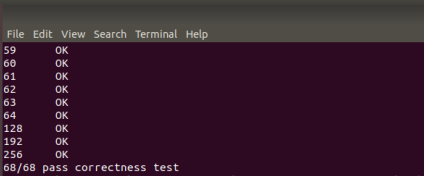
\includegraphics[width=0.95\textwidth]{pipe_correctness.png}
  \item Secondly, as shown in the figure below, the ncopy file is 948bytes, less than the required 1000bytes. \\
  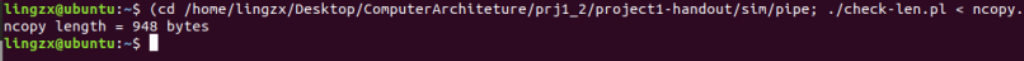
\includegraphics[width=0.95\textwidth]{pipe_checklen.png}
  \item Thirdly, as shown in the figure below, our implementation of iaddl and leave has survived all ISA checks.\\
  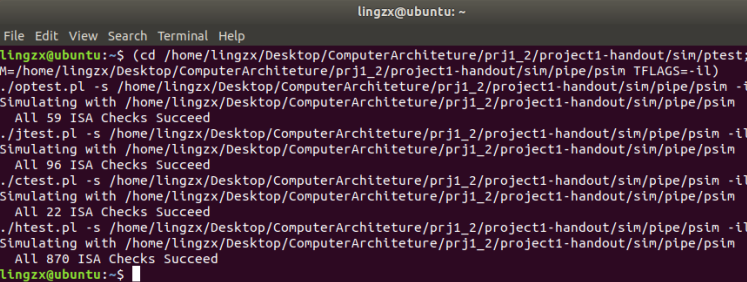
\includegraphics[width=0.95\textwidth]{pipe_ISACheck.png}
  \item Fourthly, as shown in the figure above, our ncopy function achives an average CPE of 9.89, less than 10.0, which means ncopy performs very well. As expected, the larger the number of elements is, the better the function performs. That is because when there are only several elements, loop unrolling and loose ends increase branch instructions; however, when the number is larger, the reduction of branch instructions caused by loop unrolling becomes remarkable.\\
  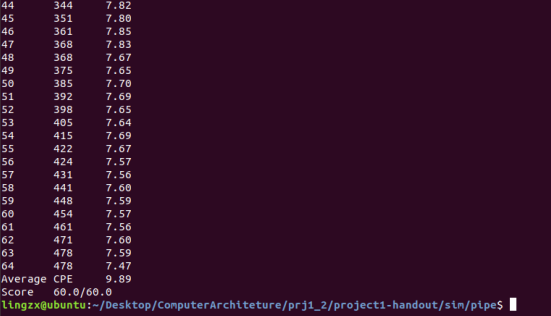
\includegraphics[width=0.95\textwidth]{pipe_CPE.png}
\end{enumerate}

\section{Conclusion}

\subsection{Problems}
There are many obstacles in the project. And we are going to share some here. \\
\begin{enumerate}

  \item Firstly, adjustment to new languages. You can never image how we feel when starting the project. It is just like language bombing. Both Y86 and HCL are new to us. And the related resources on the Internet are so poor that we have no idea how to start. However, after days of searching and thinking, we gradually adjust ourselves to the new languages. Y86 is similar to but much simpler than X86 and MIPS familiar to us. As for HCL, though more complex, the project does not require us to fully master it. It is enough if we just known how to make the logic clear. Besides, thanks to CSAPP, we can acquire a lot of related materials in the book.
  \item Secondly, debugging assembly codes run by pipeline processor. It is amazingly difficult to debug our codes running by a pipeline processor. Just as the pipeline architecture is complex, the procedure of debugging is complex, too. The codes are not finished line by line. An instruction is finished in the M or WB stage and the next several instructions are already on the way. However, this does not both us in the end. Gradually, we learn to examine the contents of states and inputs of different stages and this exactly deepens our understanding of pipeline processors.
  \item Thirdly, understanding of stack pointer. This is exactly a detail problem. In this semester, we have read a lot of assembly codes but wrote little. The stack is used when passing arguments, saving registers and calling functions. As written in the given Y86 code examples, the convention is that, on entering a function, we save the base pointer(ebp), and copy the stack pointer(esp) to the base pointer. It takes us a long time to figure out why the address of the first argument is ebp+8. And finally, by carefully observing the contents of the stack, we found when esp is copied to ebp, the stack is pushed twice: one is to save the return address and the other is to save ebp. Also, on the same problem, we spend a long time to debug our rsum function just because we pass an argument when calling the function by pushing the stack BUT forgot to pop the stack to restore the stack pointer after the function is returned.
\end{enumerate}

\subsection{Achievements}

\begin{enumerate}
  \item Firstly, it is great to see we have achieved an average CPE less than 10.0. This a result of our careful design of our logic and implementation. And all of us three members have contributed a lot in the process.
  \item Secondly, we have successfully implemented leave instruction. Leave is more complicated than iaddl, especially in the pipeline architecture because it involves necessary load-read hazard, but we have implemented it.
\end{enumerate}



%----------------------------------------------------------------------------------------


\end{document}
